\begin{figure*}[t]
\centering
\includegraphics[width=\textwidth]{images/pixelmllms_failures/failures_pixmllms_3.drawio.pdf}
\vspace{-2em}
\caption{Second shortcoming of pixel-level MLLMs is the degraded performance in pixel-level visual grounding in certain models. The predicted segmentation is highlighted in red.} 
\label{fig:shortcoming3}
\vspace{-1em}
\end{figure*}

\begin{figure}[t]
\centering
\includegraphics[width=0.5\textwidth]{images/pixelmllms_failures/failures_pixmllms_2.drawio.pdf}
\vspace{-2em}
\caption{Third shortcoming of pixel-level MLLMs is the degraded performance in instruction following, where the question is instructing the model to generate one letter from the options.} 
\label{fig:shortcoming2}
\vspace{-1em}
\end{figure}

In this section, we describe our two benchmarks and probing techniques for pixel-level MLLMs and MLLMs that were not trained with pixel-level grounding supervision.
\subsection{Benchmarks}
\textbf{PixMMVP benchmark:} We build upon the recently released MMVP~\cite{tong2024eyes} which identified clip blind pairs and used them to build a challenging benchmark with the corresponding questions and choices for 300 images. We augment the aforementioned dataset and manually annotate each question with the corresponding object of interest referring expression, e.g. an elderly person or the butterfly's feet. There are seven questions only that are not designed to inquire about a specific object in the scene, which are excluded. Examples include questions inquiring on the view direction of the camera which are not tied to a specific entity. Our manual referring expression annotations are as fine-grained as possible. These expressions correspond to what needs to be grounded in the image to answer the question. Afterwards, we manually label these objects of interest with polygonal annotations using the VGG annotator~\cite{dutta2016via}.

\textbf{PixCV-Bench benchmark:} For this benchmark we build upon the 2D component of the recently released CV-Bench~\cite{tong2024cambrian}. We specifically select the 2D component, since they are sourced from segmentation datasets (i.e., ADE20K~\cite{zhou2017scene} and COCO~\cite{lin2014microsoft}), which can be used in our proposed benchmark. However, the publicly released CV-Bench does not identify the objects in question and their corresponding segmentation. As such we use GPT-4o to parse the questions and identify the objects of interest automatically, followed by manual inspection and correction. Specifically, we collect the classes in each image from the corresponding dataset and construct a list of class choices ``1. $<$CLS1$>$, 2. $<$CLS2$>$, ...''. Then we prompt GPT-4o with the following, \textit{``Provide number only as an answer. Identify the objects of interest in the following question: $<$QUESTION$>$ ? 1. $<$CLS1$>$, 2. $<$CLS2$>$, ... ''.}  This provides us with the categories per question that highlights the objects of interest. While seemingly these are categorical annotations not referring expressions, certain scenarios in CV-Bench are different. Specifically, in the relative positioning task all the questions that include an object highlighted by a red box in the image are annotated with the referring expression, ``(annotated by the red box)'', beyond simple categorical annotations.

Afterwards, we use the selected categories from GPT-4o to retrieve the corresponding segmentation mask/s per image. Furthermore, we use a custom annotation tool to manually filter the objects in the question, e.g. selecting only the object mask annotated by the red box when referred to it and filtering out the other instances for that same class. Another example that needs manual filtration when the class in question is a broader category than what is inquired upon, e.g., ``Pendant Lamp'' which is under the category of ``Lamp'' in ADE20K. In such a case, we filter out the masks of other types such as ``Table Lamp''. Moreover, we identify missing annotations in rare occasions that require additional intervention and manually annotate these missing objects. We provide the final PixCV-Bench with referring expressions and their segmentation annotations that can be used to evaluate the grounding ability in relation to the original VQA task. Appendix~\ref{app:impdetails} provides visual examples from our benchmarks.

\subsection{A Pixel-level MLLMs study}

We utilize the two proposed benchmarks, PixMMVP and PixCV-Bench, to evaluate how the current trend in pixel-level MLLMs that relies on training with grounding supervision perform in such challenging tasks. Furthermore, we inspect the failures of these pixel-level MLLMs and explore simple approaches to pixel-level understanding from MLLMs that overcome the previous shortcomings. %We aim to answer two major research questions in our study; ``How do Pixel-level MLLMs perform in challenging pixel-level visual grounding tasks?'' and ``Whether grounding can be extracted from MLLMs that were not necessarily trained with full supervision as a simpler but more powerful means? and When does that grounding emerge?''

\textbf{Pixel-level MLLMs shortcomings.} We highlight the failures for the current state-of-the-art pixel-level MLLMs through three probing techniques. First, we highlight the degraded performance in VQA from most of the pixel-level MLLMs that are trained with pixel-level grounding supervision. We use for that the following prompt, \textit{``$<$IMG$>$$<$QUESTION$>$? $<$OPTION1$>$ $<$OPTION2$>$...''}, as shown in Figure~\ref{fig:shortcoming1}. Certain pixel-level MLLMs tend to answer the aforementioned question while outputting a corresponding segmentation mask/s for the objects of interest. Notably, the worst two models in this task, LISA~\cite{lai2024lisa} and GLAMM~\cite{rasheed2024glamm}, are not able to provide an answer and rather refer to a segmentation mask. On the other hand, OMG-Llava~\cite{zhang2024omg} shows better ability in VQA.%, yet the answer is not necessarily the correct one.

The second shortcoming we discuss is their degraded ability to visually ground objects. Surprisingly, although they were trained with pixel-level grounding supervision, not all of these models show superior grounding performance. Figure~\ref{fig:shortcoming3} shows the second prompt to generate a segmentation mask for the ground-truth referring expression. The purpose of this probing is to understand whether the failure in these models is purely on the VQA task, or its inability to ground the objects of interest in the corresponding question or both. Figure~\ref{fig:shortcoming3} shows the worst two models in this aspect, which are GLAMM, the region captioning variant, and Llava-G. Both fail to segment the specific object in question, while OMG-Llava shows better performance.

Third, we highlight another shortcoming, where these MLLMs exhibit degraded ability to follow instructions. In order to probe this, we use the following prompt: \textit{``$<$IMG$>$$<$QUESTION$>$? a.$<$OPTION1$>$ b.$<$OPTION2$>$... Answer with the option's letter from the given.''} Figure~\ref{fig:shortcoming2} shows an example with the answers from the worst two models in this aspect which are LISA~\cite{lai2024lisa} and Llava-G~\cite{zhang2025llava}. Both are incapable of following the instruction, yet Llava-G tries to tackle the question unlike LISA. On the other hand, OMG-Llava shows better ability to follow the instruction and answer the question. 

\textbf{Baselines and upper bounds.} In addition to evaluating state-of-the-art pixel-level MLLMs, we propose two baselines and one upper bound. The first of which is inspired by a concurrent work~\cite{cao2024emerging} that identified the emergent grounding in multi-modal large language models without the need for any pixel-level grounding supervision. Specifically, we use their attend and segment meta architecture as one of our baselines. However, we are the first to discuss when does such grounding emerge in these models. We identify an interesting connection between the identified output tokens and the output grounding from the attention maps that gives insights on how these models reason. 

The attend and segment meta-architecture extracts the raw attention map for the $i^{th}$ output token, $A_i \in [0, 1]^{n_{\text{layer}} \times n_{\text{head}} \times (x+hw+y+i-1)}$, where $n_{\text{layer}}, n_{\text{head}}$  are the number of layers and heads, resp. Then, $x,y$ are the number of input language tokens before and after the visual tokens respectively, while $hw$ are the height and width of the input image. Only the attention corresponding to the visual tokens of length $hw$ are used, and these attention maps are averaged across the layers and heads, resulting in $\bar{A}_i \in [0, 1]^{h \times w}$. This is further normalized across all the output, $\tilde{A}_i = \bar{A}_i - \frac{1}{N} \sum_{j=1}^{N}{\bar{A}_j}$ for $N$ output tokens. The attend and segment depends on using spaCy natural language processing tool~\cite{spaCy} to identify the noun phrases and associate them to the ground-truth referring expressions. Thus, the spaCy embeddings closest to the ground-truth expression are used in the mask selection. This is followed by extracting the maximum attention point to feed into SAM~\cite{kirillov2023segment} as a point prompt.

%\begin{table*}[t]
%\centering
%\begin{tabular}{lc|cccc|c}
%\hline
%\textbf{Method} & \textbf{PixGr. Train} & \multicolumn{4}{|c|}{\textbf{MMVP \& PixMMVP}}  \\ 
%                &                  & $\mathcal{A}\dagger$  & $\mathcal{A}$ & $\mathcal{M}\dagger$ & $\mathcal{M}$ & $\mathcal{S}$\\\hline
%Llava 1.5 (7B)~\cite{liu2024visual}  &   \xmark      &     \textbf{28.7}       & \textbf{28.0}      &     -      &     -     & -\\
%Llava 1.5 (13B)~\cite{liu2024visual} &   \xmark      &     \textbf{39.3}       & \textbf{30.0}      &     -      &     -     & -\\
%Cambrian (8B)*~\cite{tong2024cambrian}  &   \xmark   & \textbf{52.0}  & \textbf{52.0} &     -      &     -     & -\\
%OMG Llava (7B)**~\cite{zhang2024omg}  &   \checkmark   &     12.0       & 12.0      &    17.8    &     38.0  & 18.2\\
%GLAMM (7B)~\cite{rasheed2024glamm} &   \checkmark    &      1.3         &   2.7     &    \textbf{31.5}    &     \textbf{47.4}  & 5.1\\
%GLAMM - RegCap (7B)~\cite{rasheed2024glamm} &   \checkmark    &      12.7              &    6.7    &    14.5    &     18.6  & 15.1\\
%LISA (7B)~\cite{lai2024lisa}       &   \checkmark    &       7.3              &    -      &     18.1      &    42.9   & 12.5\\
%Llava-G (7B)~\cite{zhang2025llava}    &    \checkmark   &       9.3             &    -      &     17.8   &     13.5  & 12.2\\
%
%Llava 1.5 (7B) + (a+s)~\cite{cao2024emerging}  &  \xmark &      \textbf{28.7}       & \textbf{28.0} &   11.1  &  11.2 & 16.1 \\ 
%Llava 1.5 (13B) + (a+s)~\cite{cao2024emerging} &  \xmark &        \textbf{39.3}  &    \textbf{30.0}   &    9.8  &  11.4 & 17.7\\ 
%Cambrian (8B)* + (a+s)~\cite{cao2024emerging}  &  \xmark &      \textbf{52.0}            & \textbf{52.0}  &   14.3  &  15.1 & 23.4 \\ \hline
%
%PixFoundation (Llava (7B)) (Ours)    & \xmark  &     \textbf{28.7}       & \textbf{28.0} &  16.9  & 18.8 & \textbf{22.7}\\ 
%PixFoundation (Llava (13B)) (Ours)    & \xmark  &    \textbf{39.3}  &     \textbf{30.0}  &   \textbf{14.4} & \textbf{18.2} & \textbf{24.9}\\ 
%PixFoundation (Cambrian (8B)*) (Ours)    & \xmark  &  \textbf{52.0} &  \textbf{52.0}  &  \textbf{17.2}  & \textbf{18.9} & \textbf{27.7} \\ \hline
%\multicolumn{7}{l}{\textbf{Upper Bound - Oracle Selection}} \\ \hline
%PixFoundation$\dagger$ (Llava (7B)) (Ours)    & \xmark  &     28.7       & 28.0 &  \textbf{\textcolor{red}{26.1}}   & \textbf{\textcolor{red}{38.0}}   & \textcolor{red}{\textbf{32.7}}\\ 
%PixFoundation$\dagger$ (Llava (13B)) (Ours)    & \xmark  &    39.3  &   30.0  &    \textbf{\textcolor{red}{23.6}} &   \textbf{\textcolor{red}{38.2}} & \textcolor{red}{\textbf{38.7}}\\ 
%PixFoundation$\dagger$ (Cambrian (8B)*) (Ours)    & \xmark  & 52.0  & 52.0 & \textbf{\textcolor{red}{52.0}}  & \textbf{\textcolor{red}{56.1}} &  \textcolor{red}{\textbf{54.0}}\\ \hline
%\end{tabular}
%\caption{\textbf{PixMMVP} benchmark evaluation of pixel-level MLLMs and baselines. We evaluate the VQA accuracy in the first and third probing (i.e., $\mathcal{A}\dagger$ and $\mathcal{A}$ resp.). Additionally, we evaluate pixel-level visual grounding with output segmentation in the first two probing (i.e., $\mathcal{M}\dagger$ and $\mathcal{M}$ resp.). *, **: models using Llama 3 (8B) and InterLM2 (7B) respectively, unlike the rest that are relying on Vicuna (7B and 13B) for the base LLM. - : indicates either the model can not be evaluated in that setting, or has low results below 1\% showing complete failure in that setting. $\mathcal{S}$: denotes the score of the MLLM that is the harmonic mean of $\text{max}(\mathcal{A}, \mathcal{A}\dagger)$ and $\text{max}(\mathcal{M}, \mathcal{M}\dagger)$. PixGr. Train: pixel-level grounding training. The oracle results are highlighted in red, and the best in each variant (7B, 13B, and 8B) are bolded. }
%\label{tab:pixmmvp}
%\end{table*}

%\begin{table*}[t]
%\centering
%\begin{tabular}{lc|cccc|c}
%\hline
%\textbf{Method} & \textbf{PixGr. Train} & \multicolumn{4}{|c|}{\textbf{PixMMVP}}  \\ 
%                &                  & $\mathcal{A}\dagger$  & $\mathcal{A}$ & $\mathcal{M}\dagger$ & $\mathcal{M}$ & $\mathcal{S}$\\\hline
%Llava 1.5 (7B)~\cite{liu2024visual}  &   \xmark      &     \textbf{27.3}       & \textbf{28.0}      &     -      &     -     & -\\
%Llava 1.5 (13B)~\cite{liu2024visual} &   \xmark      &   \textbf{39.3}        &  \textbf{30}     &     -      &     -     & -\\
%Cambrian (8B)*~\cite{tong2024cambrian}  &   \xmark   & \textbf{52.0}  & \textbf{52.0} &     -      &     -     & -\\
%OMG Llava (7B)**~\cite{zhang2024omg}  &   \checkmark   &     12.0       & 12.0      &    17.8    &     38.0  & 18.2\\
%GLAMM (7B)~\cite{rasheed2024glamm} &   \checkmark    &      1.3         &   2.7     &    \textbf{31.5}    &     \textbf{47.4}  & 5.1\\
%GLAMM - RegCap (7B)~\cite{rasheed2024glamm} &   \checkmark    &      12.7              &    6.7    &    14.5    &     18.6  & 15.1\\
%LISA (7B)~\cite{lai2024lisa}       &   \checkmark    &       7.3              &    -      &     18.1      &    42.9   & 12.5\\
%Llava-G (7B)~\cite{zhang2025llava}    &    \checkmark   &       9.3             &    -      &     17.8   &     13.5  & 12.2\\
%
%Llava 1.5 (7B) + (a+s)~\cite{cao2024emerging}  &  \xmark &  \textbf{27.3}       & \textbf{28.0}      &   11.1  &  11.2 &  16.0\\ 
%Llava 1.5 (13B) + (a+s)~\cite{cao2024emerging} &  \xmark &  \textbf{39.3}        &  \textbf{30}    &  9.8   & 11.4  & 17.7\\ 
%Cambrian (8B)* + (a+s)~\cite{cao2024emerging}  &  \xmark &      \textbf{52.0}            & \textbf{52.0}  &   14.3  &  15.1 & 23.4 \\ \hline
%
%% Old approach using Cambrian
%%PixFoundation (Llava (7B)) (Ours)    & \xmark  &    \textbf{27.3}       & \textbf{28.0}      &  16.9  & 18.8 & \textbf{22.5}\\ 
%%PixFoundation (Llava (13B)) (Ours)    & \xmark  &   \textbf{39.3}        &  \textbf{30}     &  \textbf{14.4}  & \textbf{18.2} & \textbf{24.9} \\ 
%%PixFoundation (Cambrian (8B)*) (Ours)    & \xmark  &  \textbf{52.0} &  \textbf{52.0}  &  \textbf{17.2}  & \textbf{18.9} & \textbf{27.7} \\ \hline
%
%% new approach using GPT
%PixFoundation (Llava (7B)) (Ours)    & \xmark  &    \textbf{27.3}       & \textbf{28.0}      & 18.8  & 25.9 & \textbf{26.9}\\ 
%PixFoundation (Llava (13B)) (Ours)    & \xmark  &   \textbf{39.3}        &  \textbf{30}     &  \textbf{16.9}  & \textbf{25.0} &  \textbf{30.6}\\ 
%PixFoundation (Cambrian (8B)*) (Ours)    & \xmark  &  \textbf{52.0} &  \textbf{52.0}  &  \textbf{29.6}  &  \textbf{30.3} & \textbf{38.3} \\ \hline
%
%\multicolumn{7}{l}{\textbf{Upper Bound - Oracle Selection}} \\ \hline
%PixFoundation$\dagger$ (Llava (7B)) (Ours)    & \xmark  &    27.3  & 28.0  &  \textbf{\textcolor{red}{26.1}}   & \textbf{\textcolor{red}{38.0}}   & \textcolor{red}{\textbf{32.2}}\\ 
%PixFoundation$\dagger$ (Llava (13B)) (Ours)    & \xmark  &    39.3        &  30 &  \textbf{\textcolor{red}{23.6}}  &  \textbf{\textcolor{red}{38.2}} & \textbf{\textcolor{red}{38.7}}\\ 
%PixFoundation$\dagger$ (Cambrian (8B)*) (Ours)    & \xmark  & 52.0  & 52.0 & \textbf{\textcolor{red}{52.0}}  & \textbf{\textcolor{red}{56.1}} &  \textcolor{red}{\textbf{54.0}}\\ \hline
%\end{tabular}
%\caption{\textbf{PixMMVP} benchmark evaluation of pixel-level MLLMs and baselines. We evaluate the VQA accuracy in the first and third probing (i.e., $\mathcal{A}\dagger$ and $\mathcal{A}$ resp.). Additionally, we evaluate pixel-level visual grounding with output segmentation in the first two probing (i.e., $\mathcal{M}\dagger$ and $\mathcal{M}$ resp.). *, **: models using Llama 3 (8B) and InterLM2 (7B) respectively, unlike the rest that are relying on Vicuna (7B and 13B) for the base LLM. - : indicates either the model can not be evaluated in that setting, or has low results below 1\% showing complete failure in that setting. $\mathcal{S}$: denotes the score of the MLLM that is the harmonic mean of $\text{max}(\mathcal{A}, \mathcal{A}\dagger)$ and $\text{max}(\mathcal{M}, \mathcal{M}\dagger)$. PixGr. Train: pixel-level grounding training. The oracle results are highlighted in red, and the best in each variant (7B, 13B, and 8B) are bolded. }
%\label{tab:pixmmvp}
%\end{table*}

For our baseline and upper bound, we build upon the previous pipeline and build an \textit{oracle} upper bound and an \textit{automatic} baseline. We introduce two main modifications to account for our observation that the correct grounding can occur with different output tokens describing the object not necessarily aligning with the exact ground-truth expression. The first modification is to go through all the potential output tokens without relying on spaCy embeddings. In the \textit{oracle} we rely on the ground-truth mask to select the correct token and its corresponding attention map with highest intersection over union as an upper bound. The \textit{automatic} baseline uses a simple but powerful mechanism where we overlay the predicted masks on the original image to highlight the potential object of interest. This is followed by feeding these images to a multi-modal LLM inquiring on which is best in highlighting this object. Specifically, we use the following prompt \textit{``Select the image that has $<$EXPR$>$ best highlighted in red color than the others? Answer with a number from 1 to $<$N$>$ and mention the number only. $<$IMG$>$''}, where  $<$EXPR$>$ and $<$IMG$>$ are the ground-truth expression and the image tokens respectively. In our automatic baseline we rely on GPT-4o for the mask selection. The second modification, since SAM has a good understanding of point prompting ambiguity, we process three potential output masks for each prompt instead of one only. This enables us to utilize the power of SAM in identifying fine-grained objects and referring expressions that tends to surpass what other MLLMs do, even those trained with pixel-level grounding supervision. %These baselines serve the main purpose that the correct grounding is already embedded in these MLLMs without any grounding supervision and the \textit{oracle} upper bound shows it surpasses any other MLLM with a significant margin. Thus, our proposed benchmarks and baselines confirm that pixel-level grounding is already embedded in such MLLMs and there is still plenty of opportunity to improve the grounding output further if equipped with the right tool to identify when grounding emerges.

%\begin{table*}[t]
%\centering
%\begin{tabular}{lc|cccc|c}
%\hline
%\textbf{Method}                     & \textbf{PixGr. Train} & \multicolumn{4}{|c|}{\textbf{CV-Bench \& PixCV-Bench}} \\
%                                    &                  & $\mathcal{A}\dagger$  & $\mathcal{A}$ & $\mathcal{M}$ & $\mathcal{M}\dagger$ & $\mathcal{S}$\\\hline
%%LLava 1.5 (7B)                      & \xmark           & \textbf{52.6/66.2/59.4} & \textbf{55.0/67.5/61.3} &     -     &     -      & -\\
%%LLava 1.5 (13B)                     &  \xmark          & \textbf{51.8/65.6/59.1} & \textbf{55.6/68.7/62.1} &     -     &    -       & -\\
%Llava 1.5 (7B)~\cite{liu2024visual}  & \xmark           & 16.7/14.7/15.7 & \textbf{54.2/66.5/60.4} &     -     &     -      & -\\
%Llava 1.5 (13B)~\cite{liu2024visual}  &  \xmark          & \textbf{14.6/16.7/15.6} & \textbf{55.6/67.1/61.3} &     -     &    -       & -\\
%Cambrian (8B)*~\cite{tong2024cambrian}&\xmark          & \textbf{55.7/68.7/62.2} &  \textbf{65.2/79.1/72.2}  &     -     &     -   & -\\
%OMG Llava (7B)**~\cite{zhang2024omg}    &   \checkmark    & 9.2/14.7/12.0 & 36.8/47.4/42.1 &   -       &   50.5  & \textbf{45.9}\\%OMG LLava changed
%GLAMM (7B)~\cite{rasheed2024glamm}    &    \checkmark   &      -         &      -         &   \textbf{30.2}    & \textbf{51.9}   & -\\
%GLAMM - RCap (7B)~\cite{rasheed2024glamm} &   \checkmark    & \textbf{22.8/32.8/27.8} & 46.8/62.0/54.4 &  3.6      &  7.4  & 13.0\\
%LISA (7B)~\cite{lai2024lisa}       &   \checkmark    & 1.9/5.5/3.7  &       -        &   16.8    &  48.1     & 6.7\\ %LISA changed reflect change in finegrained analysis
%Llava-G (7B)~\cite{zhang2025llava} &    \checkmark   & 13.9/14.2/14.1 & 5.1/3.7/4.4    &    1.7    &  17.6     & 15.8\\
%
%%LLava 1.5 (7B) + (a+s)               & \xmark          & \textbf{52.6/66.2/59.4} & \textbf{55.0/67.5/61.3} &   4.7     &    14.9   & \\ 
%%LLava 1.5 (13B) + (a+s)              & \xmark          &  \textbf{51.8/65.6/59.1} & \textbf{55.6/68.7/62.1} &    5.2    &   15.7    & \\ 
%%Cambrian (8B)* + (a+s)~\cite{cao2024emerging}  & \xmark & \textbf{64.5/77.4/71.0} & \textbf{65.1/79.4/72.3} &  18.5    &   15.9    &  \\ \hline %19.3
%
%Llava 1.5 (7B) + (a+s)~\cite{cao2024emerging} & \xmark          & 16.7/14.7/15.7 & \textbf{54.2/66.5/60.4} &   5.2  & 15.6 & 24.8\\ 
%Llava 1.5 (13B) + (a+s)~\cite{cao2024emerging} & \xmark          & \textbf{14.6/16.7/15.6} & \textbf{55.6/67.1/61.3}  &  \textbf{4.7}    &    14.9    & 24.0\\ %STILL
%Cambrian (8B)* + (a+s)~\cite{cao2024emerging}  & \xmark &  \textbf{55.7/68.7/62.2} & \textbf{65.2/79.1/72.2} &  \textbf{18.6}  &    15.9  &  \textbf{29.6}\\ \hline
%
%%PixFoundation (LLava (7B)) (Ours)    & \xmark          & \textbf{52.6/66.2/59.4} & \textbf{55.0/67.5/61.3} &    5.0     &    18.7   & \\ 
%%PixFoundation (LLava (13B)) (Ours)   & \xmark          & \textbf{51.8/65.6/59.1} & \textbf{55.6/68.7/62.1} &    4.7     &     18.4  & \\ 
%%PixFoundation (Cambrian (8B)*)(Ours)  & \xmark         & \textbf{64.5/77.4/71.0} & \textbf{65.1/79.4/72.3} &    11.8     &     16.1  & \\ \hline
%
%PixFoundation (Llava (7B)) (Ours)    & \xmark          & 16.7/14.7/15.7 & \textbf{54.2/66.5/60.4} &  \textbf{5.3}     &   \textbf{19.1}  & 29.0\\ %STILL
%PixFoundation (Llava (13B)) (Ours)   & \xmark          &  \textbf{14.6/16.7/15.6} & \textbf{55.6/67.1/61.3}  &     \textbf{4.7}  &  \textbf{17.7}    & \textbf{27.5}\\ %STILL
%PixFoundation (Cambrian (8B)*)(Ours)  & \xmark         &   \textbf{55.7/68.7/62.2} &  \textbf{65.2/79.1/72.2} &    12.1    &  \textbf{16.6}    & 27.0\\ \hline %(Sun)
%
%\multicolumn{7}{l}{\textbf{Upper Bound - Oracle Selection}} \\ \hline
%%PixFoundation$\dagger$ (LLava (7B)) (Ours)    & \xmark  & 52.6/66.2/59.4 & 55.0/67.5/61.3 &    \textcolor{red}{\textbf{6.3}}    &     \textcolor{red}{\textbf{49.7}}  & 54.9\\ 
%%PixFoundation$\dagger$ (LLava (13B)) (Ours)    & \xmark & 51.8/65.6/59.1 & 55.6/68.7/62.1 &    \textcolor{red}{\textbf{5.3}}    &     \textcolor{red}{\textbf{51.7}}  & \\ 
%%PixFoundation$\dagger$ (Cambrian (8B)*) (Ours)  & \xmark & 64.5/77.4/71.0 & 65.1/79.4/72.3 &   \textcolor{red}{\textbf{54.6}}   &   \textcolor{red}{\textbf{64.5}}   & \\ \hline 
%
%PixFoundation$\dagger$ (Llava (7B)) (Ours)    & \xmark  &  16.7/14.7/15.7 & 54.2/66.5/60.4 &  \textbf{\textcolor{red}{6.3}}  &   \textbf{\textcolor{red}{49.7}}   & \textbf{\textcolor{red}{54.5}}\\ 
%PixFoundation$\dagger$ (Llava (13B)) (Ours)    & \xmark &  14.6/16.7/15.6 & 55.6/67.1/61.3  &  \textbf{\textcolor{red}{5.3}}  &   \textbf{\textcolor{red}{50.6}}   & \textbf{\textcolor{red}{55.4}}\\ 
%PixFoundation$\dagger$ (Cambrian (8B)*) (Ours)  & \xmark & 55.7/68.7/62.2 & 65.2/79.1/72.2 &   \textbf{\textcolor{red}{54.3}}    & \textbf{\textcolor{red}{64.4}}   & \textbf{\textcolor{red}{68.1}}\\ \hline
%
%\end{tabular}
%\caption{\textbf{PixCV-Bench} benchmark evaluation of the various pixel-level MLLMs and the different baselines We evaluate VQA accuracy in the first and third probing (i.e., $\mathcal{A}, \mathcal{A}\dagger$ resp.). Note, we show the accuracies as $././.$ for the ADE20K, COCO and the average of both respectively. Additionally, we evaluate pixel-level visual grounding ability with output segmentation masks in the first two probing (i.e., $\mathcal{M}\dagger, \mathcal{M}$ resp.). *, **: models using Llama 3 (8B) and InterLM2 (7B) respectively, unlike the rest that are relying on Vicuna (7B and 13B) for the base LLM. GLAMM-RCAp: is the GLAMM-RegCap variant. - : indicates either the model can not be evaluated in that setting, or has low results below 1\% showing complete failure in that setting. $\mathcal{S}$: denotes the score of the MLLM that is the harmonic mean of $\text{max}(\mathcal{A}, \mathcal{A}\dagger)$ and $\text{max}(\mathcal{M}, \mathcal{M}\dagger)$. PixGr. Train: pixel-level grounding training. The oracle results are highlighted in red, and the best in each variant (7B, 13B, and 8B) are bolded.}
%\label{tab:pixcvbench}
%\end{table*}


%\begin{table*}[t]
%\centering
%\begin{tabular}{lc|cccc|c}
%\hline
%\textbf{Method}                     & \textbf{PixGr. Train} & \multicolumn{4}{c|}{\textbf{PixCV-Bench}} \\
%                                    &                  & $\mathcal{A}\dagger$  & $\mathcal{A}$ & $\mathcal{M}$ & $\mathcal{M}\dagger$ & $\mathcal{S}$\\\hline
%Llava 1.5 (7B)~\cite{liu2024visual}  & \xmark           & 18.0/16.7/17.4 & \textbf{54.1/66.5/60.3} &     -     &     -      & -\\
%Llava 1.5 (13B)~\cite{liu2024visual}  &  \xmark          & \textbf{13.6/15.4/14.5} & \textbf{55.6/67.1/61.4}  &     -     &    -       & -\\
%Cambrian (8B)*~\cite{tong2024cambrian}&\xmark          & \textbf{55.7/68.7/62.2} &  \textbf{65.2/79.1/72.2}  &     -     &     -   & -\\
%OMG Llava (7B)**~\cite{zhang2024omg}    &   \checkmark    & 9.2/14.7/12.0 & 36.8/47.4/42.1 &   -       &   50.5  & \textbf{45.9}\\%OMG LLava changed
%GLAMM (7B)~\cite{rasheed2024glamm}    &    \checkmark   &      -         &      -         &   \textbf{30.2}    & \textbf{51.9}   & -\\
%GLAMM - RCap (7B)~\cite{rasheed2024glamm} &   \checkmark    & \textbf{22.8/32.8/27.8} & 46.8/62.0/54.4 &  3.6      &  7.4  & 13.0\\
%LISA (7B)~\cite{lai2024lisa}       &   \checkmark    & 1.9/5.5/3.7  &       -        &   16.8    &  48.1     & 6.7\\ %LISA changed reflect change in finegrained analysis
%Llava-G (7B)~\cite{zhang2025llava} &    \checkmark   & 13.9/14.2/14.1 & 5.1/3.7/4.4    &    1.7    &  17.6     & 15.8\\
%
%Llava 1.5 (7B) + (a+s)~\cite{cao2024emerging} & \xmark          & 18.0/16.7/17.4 & \textbf{54.1/66.5/60.3} &  5.2   & 15.7  & 24.9 \\ 
%Llava 1.5 (13B) + (a+s)~\cite{cao2024emerging} & \xmark          & \textbf{13.6/15.4/14.5} & \textbf{55.6/67.1/61.4}  & 4.7  &  14.9  & 
%24.0 \\ 
%Cambrian (8B)* + (a+s)~\cite{cao2024emerging}  & \xmark &  \textbf{55.7/68.7/62.2} & \textbf{65.2/79.1/72.2} &  18.6  &    15.9  &  29.6\\ \hline
%
%PixFoundation (Llava (7B)) (Ours)    & \xmark          & 18.0/16.7/17.4 & \textbf{54.1/66.5/60.3}  &  5.4  & 28.5 & 38.7\\ 
%PixFoundation (Llava (13B)) (Ours)   & \xmark          & \textbf{13.6/15.4/14.5} & \textbf{55.6/67.1/61.4}  &   \textbf{4.8} &   \textbf{27.6}   & \textbf{38.1}\\ 
%PixFoundation (Cambrian (8B)*)(Ours)  & \xmark         &   \textbf{55.7/68.7/62.2} &  \textbf{65.2/79.1/72.2} &  \textbf{23.9}   &  \textbf{33.1} & \textbf{45.4} \\ \hline %(Sun)
%
%\multicolumn{7}{l}{\textbf{Upper Bound - Oracle Selection}} \\ \hline
%
%PixFoundation$\dagger$ (Llava (7B)) (Ours)    & \xmark  &  18.0/16.7/17.4 & 54.1/66.5/60.3  &  \textbf{\textcolor{red}{6.3}}  &  \textbf{\textcolor{red}{49.7}}  & \textbf{\textcolor{red}{54.5}}\\ 
%PixFoundation$\dagger$ (Llava (13B)) (Ours)    & \xmark & 13.6/15.4/14.5 & 55.6/67.1/61.4  &  \textbf{\textcolor{red}{5.3}}  &   \textbf{\textcolor{red}{50.6}} & \textbf{\textcolor{red}{55.5}}\\ 
%PixFoundation$\dagger$ (Cambrian (8B)*) (Ours)  & \xmark & 55.7/68.7/62.2 & 65.2/79.1/72.2 &   \textbf{\textcolor{red}{54.3}}    & \textbf{\textcolor{red}{64.4}}   & \textbf{\textcolor{red}{68.1}}\\ \hline
%
%\end{tabular}
%\caption{\textbf{PixCV-Bench} benchmark evaluation of the various pixel-level MLLMs and the different baselines We evaluate VQA accuracy in the first and third probing (i.e., $\mathcal{A}, \mathcal{A}\dagger$ resp.). Note, we show the accuracies as $././.$ for the ADE20K, COCO and the average of both respectively. Additionally, we evaluate pixel-level visual grounding ability with output segmentation masks in the first two probing (i.e., $\mathcal{M}\dagger, \mathcal{M}$ resp.). *, **: models using Llama 3 (8B) and InterLM2 (7B) respectively, unlike the rest that are relying on Vicuna (7B and 13B) for the base LLM. GLAMM-RCAp: is the GLAMM-RegCap variant. - : indicates either the model can not be evaluated in that setting, or has low results below 1\% showing complete failure in that setting. $\mathcal{S}$: denotes the score of the MLLM that is the harmonic mean of $\text{max}(\mathcal{A}, \mathcal{A}\dagger)$ and $\text{max}(\mathcal{M}, \mathcal{M}\dagger)$. PixGr. Train: pixel-level grounding training. The oracle results are highlighted in red, and the best in each variant (7B, 13B, and 8B) are bolded.}
%\label{tab:pixcvbench}
%\end{table*}

\begin{table*}[t]
\centering
\begin{tabular}{lc|ccccc|ccccc}
\hline
\textbf{Method} & \textbf{PixGr.} & \multicolumn{5}{|c|}{\textbf{PixMMVP}} & \multicolumn{5}{|c}{\textbf{PixCV-Bench}}  \\ 
     &   & $\mathcal{A}\dagger$  & $\mathcal{A}$ & $\mathcal{M}\dagger$ & $\mathcal{M}$ & $\mathcal{S}$ & $\mathcal{A}\dagger$  & $\mathcal{A}$ & $\mathcal{M}\dagger$ & $\mathcal{M}$ & $\mathcal{S}$\\\hline
Llava 1.5 (7B)~\cite{liu2024visual}  &   \xmark      &     27.3       & 28.0      &     -      &     -     & -  & 17.4 & 60.3 &     -     &     -      & -\\
Llava 1.5 (13B)~\cite{liu2024visual} &   \xmark      &   39.3        &  30    &     -      &     -     & - & 14.5 & 61.4  &     -     &    -       & -\\
Cambrian (8B)*~\cite{tong2024cambrian}  &   \xmark   & 52.0  & 52.0 &     -      &     -     & - & 62.2 & 72.2  &     -     &     -   & -\\
OMG Llava (7B)**~\cite{zhang2024omg}  &   \checkmark   &     12.0       & 12.0      &    17.8    &     38.0  & 18.2  & 12.0 & 42.1 &   -       &  50.5  & \textbf{45.9}\\
GLAMM (7B)~\cite{rasheed2024glamm} &   \checkmark    &      1.3         &   2.7     &    31.5    &     47.4  & 5.1 &    -         &      -         &   30.2    & 51.9   & -\\
GLAMM - RegCap (7B)~\cite{rasheed2024glamm} &   \checkmark    &      12.7              &    6.7    &    14.5    &     18.6  & 15.1 & 27.8 & 54.4 &  3.6      &  7.4  & 13.0\\
LISA (7B)~\cite{lai2024lisa}       &   \checkmark    &       7.3              &    -      &     18.1      &    42.9   & 12.5 &  3.7  &       -        &   16.8    &  48.1     & 6.7\\
Llava-G (7B)~\cite{zhang2025llava}    &    \checkmark   &       9.3             &    -      &     17.8   &     13.5  & 12.2 & 14.1 & 4.4    &    1.7    &  17.6     & 15.8\\

Llava 1.5 (7B) + (a+s)~\cite{cao2024emerging}  &  \xmark &  27.3       & 28.0      &   11.1  &  11.2 &  16.0 &  17.4 & 60.3 &  5.2   & 15.7  & 24.9 \\ 
Llava 1.5 (13B) + (a+s)~\cite{cao2024emerging} &  \xmark &  39.3        &  30    &  9.8   & 11.4  & 17.7 & 14.5 & 61.4  & 4.7  &  14.9  & 24.0\\ 
Cambrian (8B)* + (a+s)~\cite{cao2024emerging}  &  \xmark &  52.0            & 52.0  &   14.3  &  15.1 & 23.4 &  62.2 & 72.2 &  18.6  &    15.9  &  29.6\\ \hline

% new approach using GPT
PixFoundation (7B) (Ours)    & \xmark  &    27.3       & 28.0      & 18.8  & 25.9 & 26.9 & 17.4 & 60.3  &  5.4  & 28.5 & 38.7\\ 
PixFoundation (13B) (Ours)    & \xmark  &   39.3       & 30     &  16.9  & 25.0 &  \underline{30.6} & 14.5 & 61.4  &   4.8 &   27.6   & 38.1\\ 
PixFoundation (8B)* (Ours)    & \xmark  &  52.0 &  52.0  &  29.6  &  30.3 & \textbf{38.3} & 62.2 &  72.2 &  23.9 & 33.1 & \underline{45.4}\\ \hline

\multicolumn{7}{l}{\textbf{Upper Bound - Oracle Selection}} \\ \hline
PixFoundation$\dagger$ (7B) (Ours)    & \xmark  &    27.3  & 28.0  &  \textbf{\textcolor{red}{26.1}}   & \textbf{\textcolor{red}{38.0}}   & \textcolor{red}{\textbf{32.2}} & 17.4 & 60.3  &  \textbf{\textcolor{red}{6.3}}  &  \textbf{\textcolor{red}{49.7}}  & \textbf{\textcolor{red}{54.5}}\\ 
PixFoundation$\dagger$ (13B) (Ours)    & \xmark  &    39.3        &  30 &  \textbf{\textcolor{red}{23.6}}  &  \textbf{\textcolor{red}{38.2}} & \textbf{\textcolor{red}{38.7}} & 14.5 & 61.4  &  \textbf{\textcolor{red}{5.3}}  &   \textbf{\textcolor{red}{50.6}} & \textbf{\textcolor{red}{55.5}}\\ 
PixFoundation$\dagger$ (8B)* (Ours)    & \xmark  & 52.0  & 52.0 & \textbf{\textcolor{red}{52.0}}  & \textbf{\textcolor{red}{56.1}} &  \textcolor{red}{\textbf{54.0}} & 62.2 & 72.2 &   \textbf{\textcolor{red}{54.3}}    & \textbf{\textcolor{red}{64.4}}   & \textbf{\textcolor{red}{68.1}}\\ \hline
\end{tabular}
\vspace{-0.5em}
\caption{\textbf{PixMMVP} and \textbf{PixCV-Bench} benchmark evaluation of pixel-level MLLMs and baselines. We evaluate the VQA accuracy in the first and third probing (i.e., $\mathcal{A}\dagger$ and $\mathcal{A}$ resp.). Additionally, we evaluate pixel-level visual grounding with output segmentation in the first two probing (i.e., $\mathcal{M}\dagger$ and $\mathcal{M}$ resp.). *, **: models using Llama-3-Ins (8B) and InternLM2 (7B) respectively, unlike the rest that are relying on Vicuna variants (7B and 13B) for the base LLM. - : indicates either the model can not be evaluated in that setting, or has low results below 1\% showing complete failure in that setting. $\mathcal{S}$: denotes the score of the MLLM that is the harmonic mean of $\text{max}(\mathcal{A}, \mathcal{A}\dagger)$ and $\text{max}(\mathcal{M}, \mathcal{M}\dagger)$. PixGr.: pixel-level grounding training. The oracle is highlighted in red, the best and second best in $\mathcal{S}$ is bolded and underlined resp.}
\vspace{-0.5em}
\label{tab:pixmmvp}
\end{table*}

\begin{figure*}[t]
\centering
the dorsal fin of the animal

\begin{subfigure}{0.2\textwidth}
\includegraphics[width=\textwidth]{images/qualfig1/OMGLLava/output00019.png}
\caption{OMG-Llava (7B)}
\end{subfigure}%
\begin{subfigure}{0.2\textwidth}
\includegraphics[width=\textwidth]{images/qualfig1/LISA/output00019.png}
\caption{LISA (7B)}
\end{subfigure}%
\begin{subfigure}{0.2\textwidth}
\includegraphics[width=\textwidth]{images/qualfig1/GLAMM/output00019.png}
\caption{GLAMM (7B)}
\end{subfigure}%
\begin{subfigure}{0.2\textwidth}
\includegraphics[width=\textwidth]{images/qualfig1/LLava-G/19.jpg}
\caption{Llava-G (7B)}
\end{subfigure}%
\begin{subfigure}{0.2\textwidth}
\includegraphics[width=\textwidth]{images/qualfig1/LLava157b/19.jpg}
\caption{PixFoundation$\dagger$ (7B)}
\end{subfigure}
\vspace{-1em}
\caption{\textbf{PixMMVP} qualitative comparison in pixel-level visual grounding following the second probing technique. The referred expression is shown on top. It shows that mining for the grounding within the attention maps of vanilla MLLMs using their upper bound is better than MLLMs trained with pixel-level supervision, without degrading their VQA abilities. Thus, questioning whether the current training paradigm of pixel-level MLLMs is in the right direction.} 
\vspace{-0.5em}
\label{fig:qual}
\end{figure*}

\begin{figure*}[t]
\centering
\begin{tikzpicture}
\begin{axis} [
     title={},
     width=\textwidth,
     height=.25\textheight,
     xlabel={\footnotesize \textbf{Failures}},
     ylabel={\footnotesize \textbf{Frequency}},
     bar width = 4pt,
     ybar = .01cm,
     xmin=0.0, xmax=5,
     ymin=0.0, ymax=140,
     x tick label style={font=\tiny},
     y tick label style={font=\tiny},
     xtick={1,2,3,4},
     xticklabels={VQA - Fail, Grounding - Fail, Both - Fail, Both - Success},
     y label style={at={(axis description cs:0.05,.5)},anchor=south},
     ymajorgrids=false,
     xmajorgrids=false,
     legend style={
			at={(0.5,-0.3)},
			anchor=north,
			legend columns=5,
            }
] 

\addplot[color=blue, fill=blue, area legend] coordinates{(1, 45) (2, 12) (3, 87) (4, 6)};
\addplot[color=blue!60, fill=blue!60,  area legend] coordinates {(1, 5) (2, 11) (3, 132) (4, 2)};
\addplot[color=blue!30, fill=blue!30,  area legend] coordinates {(1, 62) (2, 6) (3, 76) (4, 6)};
\addplot[color=blue!40, fill=blue!10,  area legend] coordinates {(1, 69) (2, 0) (3, 80) (4, 1)};
\addplot[color=blue!40, fill=blue!2,  area legend] coordinates {(1, 8) (2, 18) (3, 124) (4, 0)};

\addplot[color=red!20, fill=red!20,  area legend] coordinates {(1, 17) (2, 48) (3, 74) (4, 11)};
\addplot[color=red!60, fill=red!60,  area legend] coordinates {(1, 20) (2, 35) (3, 89) (4, 6)};
\addplot[color=red, fill=red,  area legend] coordinates {(1, 24) (2, 61) (3, 49) (4, 16)};

\legend{\textbf{OMG-Llava (7B)}, \textbf{Llava-G (7B)}, \textbf{LISA (7B)}, \textbf{GLaMM (7B)}, \textbf{GLaMM$\dagger$ (7B)}, \textbf{Llava (13B)}, \textbf{Llava (7B)}, \textbf{Cambrian (8B)}}

\end{axis}
\end{tikzpicture}
\caption{Frequency of failures in both visual grounding and VQA \textit{vs.} VQA failures only \textit{vs.} grounding only. Evaluation using both the first and second probing is used, the former to evaluate VQA and the later to evaluate grounding failures. For visual grounding, IoU $< 0.5$, is considered as a failure.}
\vspace{-0.5em}
\label{fig:acciou-mmvp}
\end{figure*}

\begin{figure*}[h]
\centering
\begin{subfigure}{0.48\textwidth}
\begin{tikzpicture}
\begin{axis} [
     title={},
     width=\textwidth,
     height=.2\textheight,
     xlabel={\footnotesize \textbf{Location}},
     ylabel={\footnotesize \textbf{Frequency}},
     bar width = 4pt,
     ybar = .02cm,
     xmin=-5, xmax=100,
     ymin=0.0, ymax=80,
     x tick label style={font=\tiny},
     y tick label style={font=\tiny},
     xtick={0, 10,20,30,40,50,60,70,80,90},
     y label style={at={(axis description cs:0.05,.5)},anchor=south},
     ymajorgrids=false,
     xmajorgrids=false,
     legend style={
			at={(0.5,-0.35)},
			anchor=north,
			legend columns=5,
            }
] 

%{0: 31, 1: 9, 2: 15, 3: 24, 4: 27, 5: 27, 6: 50, 7: 28, 8: 29, 9: 7}
\addplot[color=red, fill=red,  area legend] coordinates {(0, 31) (10, 9) (20, 15) (30, 24) (40, 27) (50, 27) (60, 50) (70, 28) (80, 29) (90, 7)};

%{0: 29, 1: 6, 2: 15, 3: 29, 4: 18, 5: 35, 6: 41, 7: 37, 8: 29, 9: 8}
\addplot[color=red!50, fill=red!50,  area legend] coordinates {(0, 29) (10, 6) (20, 15) (30, 29) (40, 18) (50, 35) (60, 41) (70, 37) (80, 29) (90, 8)};

%{0: 23, 1: 29, 2: 30, 3: 29, 4: 31, 5: 30, 6: 30, 7: 23, 8: 12, 9: 10}
\addplot[color=blue, fill=blue,  area legend] coordinates {(0, 23) (10, 29) (20, 30) (30, 29) (40, 31) (50, 30) (60, 30) (70, 23) (80, 12) (90, 10)};

\legend{\textbf{Llava (7B)}, \textbf{Llava (13B)},\textbf{Cambrian (8B)}}
  
\end{axis}
\end{tikzpicture}
\vspace{-1em}
\caption{}
\label{fig:tokenloc}
\end{subfigure}%
\begin{subfigure}{0.52\textwidth}
\begin{tikzpicture}
\begin{axis} [
     title={},
     width=\textwidth,
     height=.2\textheight,
     xlabel={\footnotesize \textbf{Concept}},
     ylabel={\footnotesize \textbf{Frequency}},
     bar width = 4pt,
     ybar = .02cm,
     xmin=0, xmax=7,
     ymin=0.0, ymax=200,
     xtick=data,
     x tick label style={font=\tiny,align=center},
     y tick label style={font=\tiny},
     xtick={1,2,3,4,5,6},
     xticklabels={{Colour \& \\ Appearance}, {Location \& \\ Position}, {Objects \\ Parts}, {Context}, {Objects \&\\Entities}, {State}},
     y label style={at={(axis description cs:0.05,.5)},anchor=south},
     x label style={at={(axis description cs:0.5,-.07)},anchor=north},
     ymajorgrids=false,
     xmajorgrids=false,
     legend style={
			at={(0.5,-0.45)},
			anchor=north,
			legend columns=5,
            }
] 

%{'a': 32, 'b': 21, 'c': 37, 'd': 19, 'e': 144, 'f': 3}
\addplot[color=red, fill=red,  area legend] coordinates {(1, 32) (2, 21) (3, 37) (4, 19) (5, 144) (6, 3)};

%{'a': 35, 'b': 16, 'c': 38, 'd': 17, 'e': 143, 'f': 3}
\addplot[color=red!50, fill=red!50,  area legend] coordinates {(1, 35) (2, 16) (3, 38) (4, 17) (5, 143) (6, 3)};

%{'a': 36, 'b': 15, 'c': 56, 'd': 2, 'e': 114, 'f': 25}
\addplot[color=blue, fill=blue,  area legend] coordinates {(1, 36) (2, 15) (3, 56) (4, 2) (5, 114) (6, 25)};

\legend{\textbf{Llava (7B)}, \textbf{Llava (13B)},\textbf{Cambrian (8B)}}
  
\end{axis}
\end{tikzpicture}
\vspace{-1em}
\caption{}
\label{fig:tokenconcept}
\end{subfigure}
\vspace{-2em}
\caption{Analysis on when grounding emerges on PixMMVP benchmark using the three base MLLMs, Llava 1.5 (7, 13B) and Cambrian-1 (8B), that were not trained with pixel-level grounding supervision. We follow the second probing then report the oracle selection. Analysis on: (a) the output location and (b) the output concept category, that coincides with the best segmentation.}
\vspace{-0.5em}
\label{tab:When_MMVP}
\end{figure*}

\begin{figure*}[t]
\begin{minipage}{\textwidth}
\centering
\begin{tabular}{l|llll}
\hline
\textbf{Image} & \textbf{Prompt} & \textbf{Concept Category} & \textbf{Noun Phrase} & \textbf{Output} \\ \hline
1 & \makecell[l]{Identify the butterfly's wings \\in the scene.} & Color \& Appearance & orange wings & \makecell[l]{In the image, there is a\\ butterfly with\\ orange wings.}\\
3 & \makecell[l]{Identify the flame of the match\\ in the scene.} & Location \& Position & the top & \makecell[l]{The flame of the match\\ is located at the top\\ of the image, surrounded\\ by darkness.}\\
6 & \makecell[l]{Identify the dog's face\\ in the scene.} & Color \& Appearance & a black and white dog & \makecell[l]{The dog's face in the\\ scene is a black and white\\ dog with a black nose.} \\
161 & \makecell[l]{Identify the minute hand\\ of the clock\\ in the scene.} & Location \& Position & the 12 o'clock position & \makecell[l]{The minute hand of the\\ clock in the scene is\\ located at the 12 o'clock\\ position.} \\ 
%292 & \makecell[l]{Identify the minion\\ in the image\\ smiling with its tongue out\\ in the scene.} & Color \& Appearance & a yellow shirt & \makecell[l]{The minion in the image\\ is smiling with its\\ tongue out, wearing\\ a blue overalls and\\ a yellow shirt.}
\\ \hline
\end{tabular}
\end{minipage}

\begin{minipage}{\textwidth}
\centering
\begin{subfigure}{0.2\textwidth}
\stackunder[5pt]{\includegraphics[width=\textwidth]{images/appqualwhen/1_overlays/1_002_002.jpg}}{1}
\end{subfigure}%
\begin{subfigure}{0.2\textwidth}
\stackunder[5pt]{\includegraphics[width=\textwidth]{images/appqualwhen/3_overlays/3_002_000.jpg}}{3}
\end{subfigure}%
\begin{subfigure}{0.2\textwidth}
\stackunder[5pt]{\includegraphics[width=\textwidth]{images/appqualwhen/6_overlays/6_002_000.jpg}}{6}
\end{subfigure}%
\begin{subfigure}{0.2\textwidth}
\stackunder[5pt]{\includegraphics[width=\textwidth]{images/appqualwhen/161_overlays/161_003_001.jpg}}{161}
\end{subfigure}%
%\begin{subfigure}{0.19\textwidth}
%\stackunder[5pt]{\includegraphics[width=\textwidth]{images/appqualwhen/raw_images/292.jpg}}{292}
%\end{subfigure}
\end{minipage}
\caption{Examples of noun phrases and concept categories where the grounding emerged following the second probing on PixMMVP using Llava 1.5 (7B). Predicted segmentation highlighted in red.}
\label{fig:when_imgs}
\vspace{-1em}
\end{figure*}